\documentclass[11pt,a4paper]{amsart}

\usepackage[margin=1in]{geometry}
\usepackage{graphicx}
\usepackage{amsmath}
\usepackage{amsfonts}
\usepackage{amsthm}
\usepackage{mathrsfs}
\usepackage{float}
\usepackage{subfig}
\usepackage{hyperref}
\usepackage{dsfont}



\newtheorem{thm}{Theorem}[section]
\newtheorem{ex}{Example}
\newtheorem{prb}{Problem}
\newtheorem{pf}{Proof}
\newtheorem{lem}[thm]{Lemma}
\newtheorem{prop}[thm]{Proposition}
\newtheorem{cor}[thm]{Corollary}
\newtheorem{conj}[thm]{Conjecture}
\newtheorem{defn}{Definition}[section]
\newtheorem{example}{Example}[section]

\newcommand{\PP}{\mathbb{P}}		%Used for probabilities.
\newcommand{\NN}{\mathbb{N}}		%Used to denote the natural numbers.
\newcommand{\RR}{\mathbb{R}}		%Used to denote the real numbers.
\newcommand{\statespace}{\mathscr{S}}	%Used to denote the state space.
\newcommand{\MM}{\mathscr{M}}		%Used to denote the space of measurable sets.
\newcommand{\CC}{\mathbb{C}}
\DeclareMathOperator{\Var}{\text{Var}}
\newcommand{\s}{\sigma}
\newcommand{\W}{\widetilde{W}}
\newcommand{\w}{\omega}
\newcommand{\EE}{\mathbb{E}}
\newcommand{\N}{\mathcal{N}}


\begin{document}
\title{Monte Carlo Methods: HW 3}
\author{Terrence Alsup}
\date{March 27th, 2019}
\maketitle

\emph{Note: The MCMC methods are implemented in the Python file {\tt IsingSamplers.py}}.

\vspace{0.5in}

%%%%%%%%%%%%%%%%%%%%%%%%%%%%%%%%%%%%%%

{\bf Exercise 39}\\
\\
\par The Python file {\tt IsingSamplers.py} contains a function called {\tt IsingSampler} which can be called with the option to use Gibbs sampling by repeatedly calling the function {\tt GibbsUpdate}, which is just a single step in the Markov chain.  Given a length $N$ of the chain we can obtain an approximate sample of the 2D Ising model with distribution
\[
\pi(\sigma) = \frac{1}{Z} \exp\left(  \beta \sum_{\vec{i} \leftrightarrow \vec{j}} \sigma_{\vec{i}}\ \sigma_{\vec{j}} \right)
\]
Here $\beta \propto T^{-1}$ is the inverse temperature and each $\vec{i} \in \mathbb{Z}_L^2$.  When $\beta > 0$ this is a model for ferromagnets.  The configurations with the highest probability are the ones where all spins $\sigma_{\vec{i}}$ are the same.  If $\beta < 0$, then this is a model for anti-ferromagnets, where the most likely configurations are the ones in which all of the spins are opposite of their neighbors (checkerboard pattern).  We can check how this model behaves for different $\beta$ by examining the magnetization of the lattice
\[
f(\sigma) = \sum_{\vec{i} \in \mathbb{Z}_L^2} \sigma_{\vec{i}}
\]
Figures~\ref{fig:maghistb1} and \ref{fig:maghistb005} below show histograms of the average magnetization (normalized between $-1$ and $1$) for two different values of $\beta$.  At $\beta \approx 0.44$ (see \cite{IsingWiki}) there is a phase transition where spontaneous magnetization can occur.  If the temperature is low enough, meaning $\beta \gg 0.44$, then eventually all spins will become aligned with very high probability as shown in Figure~\ref{fig:maghistb1}.  On the other hand, for sub-critical $\beta$, meaning high temperatures, the spins are almost independent.  In this regime, by the central limit theorem, the magnetization has approximately a Gaussian distribution which is shown in Figure~\ref{fig:maghistb005}.



\begin{figure}[H]
\centering
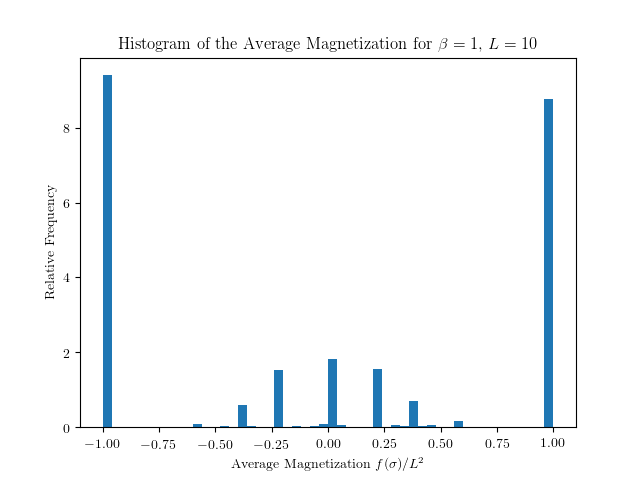
\includegraphics[width=5in]{maghistb1.png}
\caption{A histogram of 1000 samples of the average magnetization from the 2D Ising Model.  Gibbs sampling was used with the length of each chain being 10000 steps.  The lattice site to update at each step was chosen randomly.}
\label{fig:maghistb1}
\end{figure}

\begin{figure}[H]
\centering
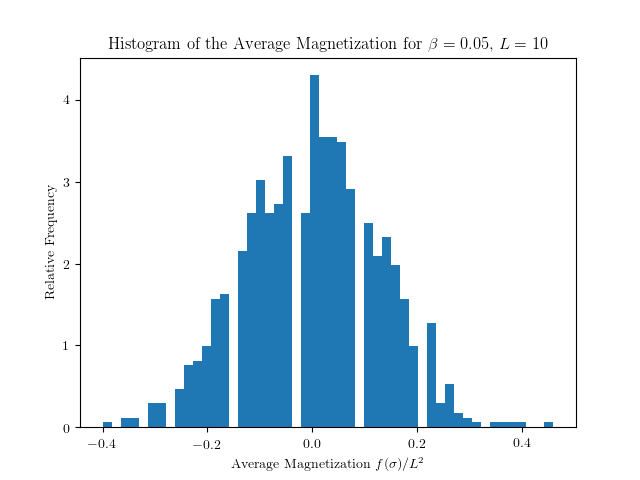
\includegraphics[width=5in]{maghistb005.png}
\caption{A histogram of 1000 samples of the average magnetization from the 2D Ising Model.  Gibbs sampling was used with the length of each chain being 10000 steps.  The lattice site to update at each step was chosen randomly.}
\label{fig:maghistb005}
\end{figure}


\par To determine how good our sampler is we can estimate the integrated autocorrelation time (IAC) $\tau$ of the magnetization. To estimate $\tau$ we use the Python package {\tt acor}.  Figure~\ref{fig:gibbsRandomACFb005} below shows the autocorrelation function of the magnetization.  We see that when $L = 10$ and $\beta = 0.05$ it takes $\approx 700$ Gibbs steps for the correlation to decay to 0.  Because after this point the noise dominates our estimate, we truncate our calculation of the IAC
\[
\hat{\tau} = 1+ 2\sum_{k=1}^{700}\text{corr}_{\pi}(f(X^{(0)}),\  f(X^{(k)}))
\]
We compute $\hat{\tau}$ for chains of length $10^{5},10^6$, and $10^7$ to see that it converges to $\tau \approx 320$.  By the same procedure, we estimate that $\hat{\tau} \approx 165$ if we instead sweep through the sites left-to-right and top-to-bottom deterministically, which is much better.  In particular, it means our effective sample size is twice as large for a fixed chain length whenever we sweep through deterministically.

\begin{figure}[H]
\centering
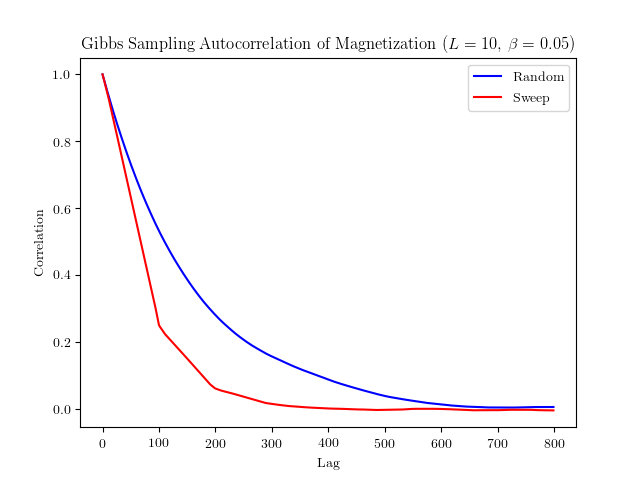
\includegraphics[width=5in]{gibbsRandomACFb005.png}
\caption{The estimated autocorrelation function of the magnetization using Gibbs sampling.  The length of the chain was $10^6$, but we truncate for a maximum lag of 800, after which point the noise begins to accumulate.  The correlation for a deterministic sweep decays much faster.}
\label{fig:gibbsRandomACFb005}
\end{figure}

\par We can also look at the dependence of the IAC on the size of the lattice $L$.  In order to get a reasonably accurate estimate of $\tau$ for $L=10$ we had to run a very long chain $10^7$.  Therefore, we only look at lattice sizes less than $12$ as shown in Figure~\ref{fig:IACL} below.  Indeed, we see that as the lattice grows in size, the longer it takes for our chain to decorrelate.  A lattice of size $L$ has $L^2$ spins and we require more than $L^2$ steps to have visited all of the sites on average at least once.  Thus, it makes sense that the IAC should increase with the size of the lattice.  In addition to changing the size of the lattice, we can also change the temperature (equivalently change $\beta$) to study the IAC.  We have already noted that there is a critical temperature where a phase transition occurs.  For larger $\beta$ (hence lower temperatures), we expect there to be magnetization as the chain moves towards a configuration where all spins are nearly the same.  When this happens any single site is unlikely to change at a given step and we expect that the IAC will grow quickly with $\beta$.  This makes it much harder to estimate the IAC for larger $\beta$.  Figure~\ref{fig:ACFb} below shows that the autocorrelation function decays extremely slowly when $\beta=1$.  We see that the scale of the $x$-axis is much larger than before.  By looking at the area under the curve, we heuristcally estimate that $\hat{\tau} \approx 750$.  Of course the variance of this estimate is so large that it is unreliable.  Regardless, we see that increasing $\beta$ (lowering the temperature) makes it much harder to sample from the Ising model.




\begin{figure}[H]
\centering
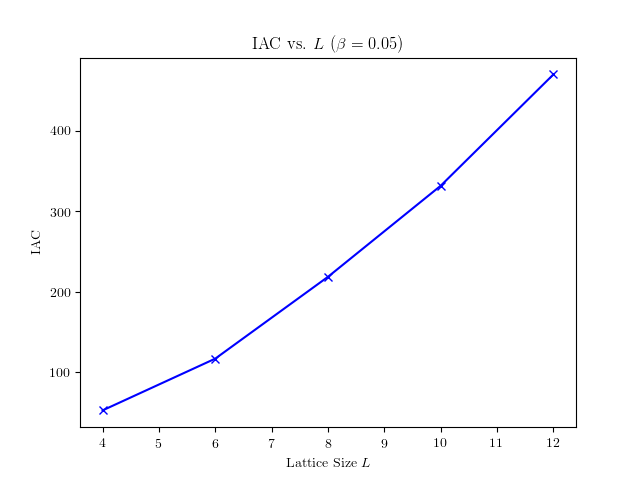
\includegraphics[width=5in]{IACL.png}
\caption{The estimated IAC of the magnetization using Gibbs sampling with random selection of the sites.  The length of the chain was $10^7$, but we truncate for a maximum lag of 700 in our estimate.}
\label{fig:IACL}
\end{figure}


\begin{figure}[H]
\centering
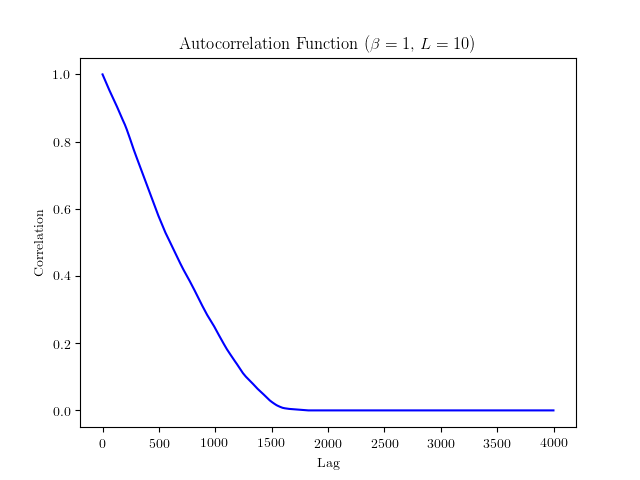
\includegraphics[width=5in]{ACFb.png}
\caption{The estimated autocorrelation function of the magnetization using Gibbs sampling with random selection of the sites.  The length of the chain was $10^6$, but we truncate the lag at 4000 for our estimate.}
\label{fig:ACFb}
\end{figure}








%%%%%%%%%%%%%%%%%%%%%%%%%%%%%%%%%%%%%%

{\bf Exercise 42}\\
\\
\par The same function {\tt IsingSampler} can instead be called to use a Metropolis-Hastings scheme.  The scheme is implemented with a proposal that randomly selects a site on the lattice and flips the sign of the spin.  Because the proposal is symmetric, the acceptance probability is then
\[
\frac{\pi(Y^{(k+1)})}{\pi(X^{(k)})} = 1 \wedge \exp \left( -4\beta X_{\vec{i}_k}(k) \sum_{\vec{j} \leftrightarrow \vec{i}_k} X_{\vec{j}}(k) \right)
\]
Figure~\ref{fig:gibbsMHACF} below compares the autocorrelation function of the Gibbs and Metropolis schemes whenever the sites are chosen randomly.  The IAC of the Metropolis scheme was computed by running chains of length $10^5$, $10^6$, and $10^7$ to check for convergence and is $\hat{\tau} \approx 189$.  This is much less than the IAC for Gibbs sampling with random selection of the sites, but is comparable to Gibbs sampling with deterministically sweeping over the sites.  For the Metropolis scheme we do not do the deterministic sweeping because then the proposal will no longer be symmetric and the acceptance probability will be much more complicated to compute.

\begin{figure}[H]
\centering
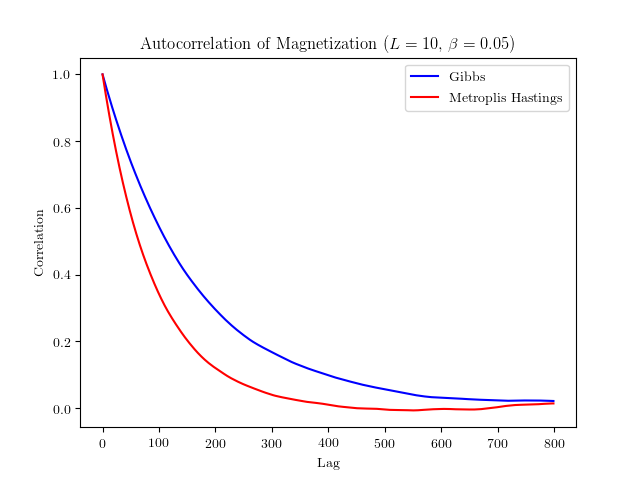
\includegraphics[width=5in]{gibbsMHACF.png}
\caption{The estimated autocorrelation functions of the magnetization.  The length of the chain was $10^7$, but we truncate for a maximum lag of 800, after which point the noise begins to accumulate.  The correlation for Metropolis-Hastings decays faster.}
\label{fig:gibbsMHACF}
\end{figure}



%%%%%%%%%%%%%%%%%%%%%%%%%%%%%%%%%%%%%%

{\bf Exercise 43}\\
\\
\par The Python file {\tt IsingSamplers.py} also contains a function called {\tt Jarzynski} which implements Jarzynski's method to compute weighted samples of the 2D Ising model as well as the option to perform resampling at each step.  We interpolate between the uniform distribution $\pi_0 \propto 1$ on $\mathbb{Z}_L^2$ to the distribution $\pi$ of the Ising model with
\[
\pi_k = \pi^{\frac{k}{N}} \propto \exp\left(  \frac{k\beta}{N} \sum_{\vec{i} \leftrightarrow \vec{j}} \sigma_{\vec{i}}\ \sigma_{\vec{j}}  \right)
\]
Initially, it is as though we were sampling the Ising model at high temperatures ($\beta \approx 0$).  Over time we lower the temperature to the get samples from $\pi$.  We implement this method with each transition operator $T_k$ being 200 Metropolis steps with $\beta \left(\frac{k-1}{N}\right)$, which preserves $\pi_{k-1}$.  We choose 200 steps since it is slightly larger than the IAC we calculated for the Metropolis scheme earlier.  We would expect that if we increase $N$ then we can obtain better estimates for the magnetization.  We use an ensemble of $M = 25$ particles with $N=10$ to compute a weighted average of the magnetization, which is our estimator.  This is done without resampling.  By symmetry the true mean magnetization is 0.  We repeat this for 100 trials and output the mean of all the trials as well as the variance of all the trials.  We computed that when $L=10$ and $\beta = 0.05$ the variance of our estimator is approximately $\hat{\sigma}^2 \approx 2.36$, which is very good consider the magnetization ranges from $\pm L^2 = \pm 100$.  In a similar manner, we also estimate the effective sample size via
\[
M_{\text{eff}} = \frac{1}{\sum_{j=1}^M W(X_j)^2}
\]
and look at the ratio $M_{\text{eff}}/M$.  We compute that $M_{\text{eff}}/M \approx 0.98$, meaning the weights are almost uniform and helps explain the low variance of our estimator.  In short, this estimator performs very well.
\\
\\

\par As we have already mentioned this procedure should be better suited for handling larger $\beta$.  To illustrate this, we increase $\beta = 1$ and examine how the variance changes with $N$.  Again we use $M=25$ particles with and without resampling and $100$ trials.  Figure~\ref{fig:varvsN} below shows the variance of the estimator as we increase the number of interpolation points $N$.  Indeed the variance decreases as we increase the number of steps.  Of course, between $\pi_{k-1}$ and $\pi_k$ remember that we do $200$ Metropolis steps.  At about $N=25$ we see that the variance begins to level-off and we get diminishing returns for increasing $N$.  Therefore, $N=25$ appears to be the optimal trade-off between computation done and performance of the estimator.  We also see that resampling only helps when $N$ is relatively small.  This is reasonable though because our effective sample size will be extremely small without resampling and the variance will be much larger.  In particular, for smaller $N$ we sample at lower temperatures, which we have already noted is much harder.

\begin{figure}[H]
\centering
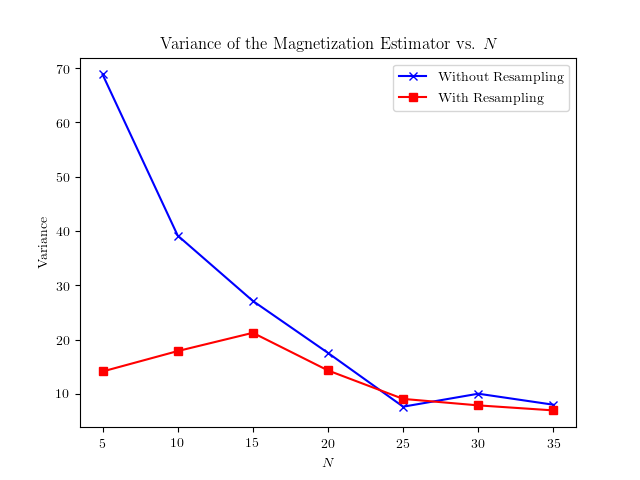
\includegraphics[width=5in]{varvsN.png}
\caption{The variance of the estimator of the mean magnetization (estimated over 100 trials) with and without resampling.}
\label{fig:varvsN}
\end{figure}

\par The most reasonable way to compare Jarzynski's method to either the Gibbs of Metropolis sampling is to analyze the effective sample sizes per number of Metropolis (or Gibbs) steps.  We know that for a chain of length $N_{\text{chain}}$ the effective sample size is $N_{\text{chain}}/\tau$.  Thus, per step the effective sample size is $1/\tau$.  For our implementation of Jarzynski's method, the total number of Metropolis steps is $M \times N \times 200$ and the effective sample size is $M_{\text{eff}}$.  Thus, we should compare, $1/\hat{\tau}$ and $M_{\text{eff}}/(M\times N \times 200)$.  For $\beta = 0.05$ we have already estimated that $\tau \approx 189$ for the Metropolis scheme.  Similarly, we estimated for Jarzynski that when $N=10$ and $M=25$ we had $M_{\text{eff}}/M \approx 0.98$, so just a regular Metropolis scheme would be more efficient.  Of course $\beta = 0.05$ is an easy problem.  For $\beta = 1$ or larger we have seen that we cannot easily estimate the IAC since the variance is huge.  On the other hand it is much easier to use Jarzynski to sample at this temperature.  The key is to get the right trade-off between accuracy and computational efficiency.





%%%%%%%%%%%%%%%%%%%%%%%%%%%%%%%%%%%%%%

\begin{thebibliography}{10}

\bibitem{IsingWiki}
Square-lattice Ising Model.\\
\texttt{https://en.wikipedia.org/wiki/Square-lattice\_Ising\_model}

\vspace{0.1in}

\bibitem{Liu}
Jun Liu (2004). \emph{Monte Carlo Strategies in Scientific Computing}.

\end{thebibliography}

%%%%%%%%%%%%%%%%%%%%%%%%%%%%%%%%%%%%%%

\end{document}
